\documentclass[twoside]{article}
\usepackage{../../estilo-ejercicios}
\newcommand{\colapso}{{\searrow\!\!\!\!\searrow}}
%--------------------------------------------------------
\begin{document}

\title{Ejercicios de Homología Simplicial}
\author{Javier Aguilar Martín, Diego Pedraza López}
\maketitle

\begin{ejercicio}{2.1}
Probar que si $K$ es un complejo simplicial conexo, entonces
$\Ima[∂_1 : C_1(K; \F) → C_0(K; \F)]$ es el subespacio de todas las cadenas $∑λ_iv_i$ con $∑λ_i = 0$.
Deducir que $H_0(K; \F) \cong \F$ generado por la clase de homología de cualquier vértice de $K$.
\end{ejercicio}
\begin{solucion}
Si $C_1(K;\F)$ está generado por $\{(v_i,v_j)\}_{i,j\in I}$, $\Ima\partial_1$ estará generado por las imágenes de estos generadores, que son expresiones de la forma $v_j-v_i$. Cualquier combinación lineal de estas expresiones nos da una cadena de la forma buscada. Si $K$ no es conexo no hay tanta diferencia, pues $C_1(K;\F)=\oplus C_1(K_i;\F)$ donde $K_i$ son las componentes conexas de $K$, de modo que de cada sumando obtendremos combinaciones $∑λ_iv_i$ con $∑λ_i = 0$, que al sumarse siguen dando una combinación de la misma forma. La diferencia está en que ahora los vértices de cada componente conexa estarían agrupados en sumandos distintos, lo que hace que la dimensión de $H_0(K;\F)$ sea igual al número de componentes conexas.

Una alternativa es recordar que $\Ima\partial_1=\ker\varepsilon$, donde $\varepsilon(v_i)=1$, al ser la homología reducida de un conexo nula, por lo que $\ker\varepsilon=\{\sum\lambda_iv_i\mid \varepsilon(\sum\lambda_iv_i)=0\}=\{\sum\lambda_iv_i\mid \sum\lambda_i =0\}$.

Comprobemos que el subespacio de tales cadenas tiene dimensión 1, de donde se deducirá el resultado. Consideremos el morfismo $C_0(K;\F)\to\F$ que a cada combinación lineal $∑λ_iv_i$ le asigna el valor de la suma $∑λ_i$. Claramente estamos buscando la dimensión del núcleo de esta aplicación, que será 0 o 1. Como hay sumas con coeficientes no nulos que verifican $∑λ_i = 0$, la dimensión no es 0, por lo que efectivamente es 1.
\end{solucion}

\newpage

\begin{ejercicio}{2.2}
Probar que $\widetilde{H}_0(K; \F) = \ker[c_∗ : H_0(K; \F) → H_0(\{v\}; \F)]$ donde $c : K →
\{v\}$ es la aplicación constante. Deducir $H_0(K; \F) \cong \widetilde{H}_0(K; \F)
⊕\F$.
\end{ejercicio}
\begin{solucion}
Se tiene que $H_0(\{v\}; \F)\cong \F\gene{v}$ y $c_*$ es la aplicación $\lambda[v_i]\mapsto \lambda [v]$, luego 
\begin{gather*}
\ker{c_*}=\{\sum\lambda_i[v_i]\mid c_*(\sum\lambda_i[v_i])=0\}=\{\sum\lambda_i[v_i]\mid \sum\lambda_ic_*[v_i]=0\}=\\
\{\sum\lambda_i[v_i]\mid\sum\lambda_i[v]=0\}=\{\sum\lambda_i[v_i]\mid \sum\lambda_i=0\}=\{[\sum\lambda_iv_i]\mid \sum\lambda_i=0\}
\end{gather*} 
Atendiendo al ejercicio anterior esto es justamente $\ker\varepsilon/\Ima\partial_1=\widetilde{H}_0$.
Del resultado anterior podemos establecer la sucesión exacta corta
\[
0\to \widetilde{H}_0(K;\F)\hookrightarrow H_0(K;\F)\overset{c_*}{\to} \F\to 0
\]
de donde se obtiene el resultado. 
\end{solucion}


\newpage

\begin{ejercicio}{2.3}
Probar que si $K_1, \dots , K_s$ son las componentes conexas de $K$, entonces
para cualquier $p ≥ 0$, $H_p(K; \F) \cong
⊕^s_{i=1}
H_p(K_i; \F)$, siendo los generadores de $H_0(K; \F)$ las
clases de homología de un vértice cualquiera por cada componente
\end{ejercicio}
\begin{solucion}
Por inducción en el número de componentes conexas es consecuencia inmediata de aplicar Mayer-Vietoris a una descomposición de $K$ como unión de una componente conexa y la unión de las demás, pues la intersección es vacía.
\end{solucion}

\newpage

\begin{ejercicio}{2.4}
Dar un ejemplo de dos complejos simpliciales no simplicialmente isomorfos
pero que tengan sus homologías isomorfas.
\end{ejercicio}
\begin{solucion}
$\{v_0,v_1,v_2,v_3,(v_0,v_1),(v_0,v_2), (v_0,v_3), (v_1,v_2)\}$ y $\{v_0,v_1,v_2,(v_0,v_1),(v_0,v_2), (v_1,v_2)\}$.
\end{solucion}

\newpage

\begin{ejercicio}{2.5}
Probar que para todo $p ≥ 0$, se tiene
\[
C_p(K; \F) \cong Z_p(K; \F)
⊕B_{p−1}(K; \F)
\]
y deducir
\[
C_p(K; \F)/B_p(K; \F) \cong H_p(K; \F)
⊕B_{p−1}(K; \F).
\]
\end{ejercicio}
\begin{solucion}
El primer resultado se tiene de la sucesión exacta
\[
0\to Z_p(K; \F)\hookrightarrow C_p(K; \F)\overset{\partial}{\to} B_{p−1}(K; \F)\to 0.
\]
Como estamos trabajando con espacios vectoriales, podemos usar que $B_p(K; \F)\cong B_p(K;\F)\oplus 0$ para decir que
\[
C_p(K; \F)/B_p(K; \F)\cong C_p(K; \F)/(B_p(K; \F)\oplus 0)\cong (Z_p(K; \F)
⊕B_{p−1}(K; \F))/(B_p(K; \F)\oplus 0)\cong H_p(K; \F)
⊕B_{p−1}(K; \F).
\]
\end{solucion}

\newpage

\begin{ejercicio}{2.6}
Sea $K$ un complejo simplicial y $K^m$ su $m$-esqueleto. Probar que $H^n(K; \F) =
H^n(K^m; \F)$ si $n < m$. ¿Qué relación hay entre $H^m(K; \F)$ y $H^m(K^m; \F)$?

\end{ejercicio}
\begin{solucion}

\end{solucion}

\newpage

\begin{ejercicio}{2.7}
Dado un complejo simplicial $K$, probar que $H_n(ΣK) \cong H_{n−1}(K)$ para
todo $n ≥ 0$.

\end{ejercicio}
\begin{solucion}

\end{solucion}

\newpage

\begin{ejercicio}{2.8}
Sea $G$ un grafo orientado y $e_1, \dots , e_µ$ aristas tales que $T = G−\{e_1, \dots , e_µ\}$
es un árbol maximal. Se denotará por $T+e_i$ al grafo $T∪\{e_i\}$. Dicho grafo contiene un único
lazo $l_i$, al cual se le puede asociar un 1-ciclo $z_i$, formado por las aristas de $l_i$ con coeficientes
$±1$, segúnn la orientación inducida por el recorrido de $l_i$ coincida con la orientación asignada
en $z_i$ para que $e_i$ aparezca con coeficiente $+1$. Prueba que $\{z_1, \dots , z_µ\}$ es una base para
$H_1(G; \F)$. Es decir, $H_1(G; \F) \cong ⊕_{µ(G)}\F$. Deduce que si $G$ es conexo con $µ(G) = 1$ entonces
$G$ tiene un único lazo.
\end{ejercicio}
\begin{solucion}

\end{solucion}

\newpage

\begin{ejercicio}{2.9}
Calcular los F-espacios vectoriales de homología de $K$, siendo $K =
\partial\sigma^n
∨
\partial σ^m$
\end{ejercicio}
\begin{solucion}

\end{solucion}

\newpage

\begin{ejercicio}{2.10}
Obtener los $\F$-espacios vectoriales de homología del complejo abstracto
$C$ correspondiente a la triangulación del cilindro vista en clase.
\end{ejercicio}
\begin{solucion}
El mismo cálculo hecho en los apuntes es válido.
\end{solucion}

\newpage

\begin{ejercicio}{2.11}
Calcular los $\F$-espacios vectoriales de homologíaa del complejo abstracto
$M$ correspondiente a la triangulación de la banda de Möbius vista en clase.
\end{ejercicio}
\begin{solucion}
El mismo cálculo hecho en los apuntes es válido.
\end{solucion}

\newpage

\begin{ejercicio}{2.12}
Demostrar que la homología simplicial (reducida) con coeficientes en
cualquier cuerpo $\F$ de la triangulación $L$ del sombrero bobo vista en clase es trivial. Sin
embargo, comprobar que $L$ no es colapsable.
\end{ejercicio}
\begin{solucion}


$L$ no es colapsable porque no tiene caras libres
\end{solucion}

\newpage

\begin{ejercicio}{2.13}
Sea $σ$ un $n$-símplice y $K$ el complejo formado por $σ$ y sus caras. Probar
que si $0 < q < n$, $H_q(K^q
; \F)$ es un $\F$-espacio vectorial de dimensión $\binom{n}
{q+1}$.
\end{ejercicio}
\begin{solucion}

\end{solucion}

\newpage

\begin{ejercicio}{2.14}
Calcular los $\F$-espacios vectoriales de homología de $K$, siendo $K$ la triangulación
del toro con una membrana vista en clase.
\end{ejercicio}
\begin{solucion}

\end{solucion}

\newpage

\begin{ejercicio}{2.15}
Triangular el espacio $X ⊆ \R^2$
consistente en $k$ circunferencias disjuntas
$S_1, \dots , S_k$ y un segmento $A$ tangente a cada una de ellas y calcular sus $\F$-espacios
vectoriales de homología.
\end{ejercicio}
\begin{solucion}\

\begin{center}
\begin{tikzpicture}[line cap=round,line join=round,>=triangle 45,x=0.7cm,y=0.7cm]
\clip(.,-1) rectangle (21.,4);
\draw[line width=2.pt] (0.,0.) -- (2.,3.) -- (4.,0.) -- cycle;
\draw[line width=2.pt] (5.,0.) -- (7.,3.) -- (9.,0.) -- cycle;
\draw[line width=2.pt] (14.,0.) -- (16.,3.) -- (18.,0.) -- cycle;
\draw [line width=2.pt] (0.,0.)-- (2.,3.);
\draw [line width=2.pt] (2.,3.)-- (4.,0.);
\draw [line width=2.pt] (4.,0.)-- (0.,0.);
\draw [line width=2.pt] (5.,0.)-- (7.,3.);
\draw [line width=2.pt] (7.,3.)-- (9.,0.);
\draw [line width=2.pt] (9.,0.)-- (5.,0.);
\draw [line width=2.pt] (14.,0.)-- (16.,3.);
\draw [line width=2.pt] (16.,3.)-- (18.,0.);
\draw [line width=2.pt] (18.,0.)-- (14.,0.);
\draw [line width=2.pt] (2.,3.)-- (16.,3.);
\draw (9.74,4.) node[anchor=north west] {$A$};
\draw (1.54,0.) node[anchor=north west] {$S_1$};
\draw (6.7,0.) node[anchor=north west] {$S_2$};
\draw (15.72,0.) node[anchor=north west] {$S_k$};
\begin{scriptsize}
\draw [fill=black] (11.,1.58) circle (1.0pt);
\draw [fill=black] (13.,1.56) circle (1.0pt);
\draw [fill=black] (12.02,1.56) circle (1.0pt);
\end{scriptsize}
\end{tikzpicture}
\end{center}

Este espacio es claramente del mismo tipo de homotopía de un wedge de circunferencias, por lo que su homología es la suma directa de las homologías de las circunferencias, que ya las conocemos.
\end{solucion}

\newpage

\begin{ejercicio}{2.16}
Dados los conjuntos de $\R
^3$
\[
A = \{(x, y, z); x^2 + y^2 + z^2 = 1, x ≤ 0\}\]
\[
B = \{(x, y, z) ∈ \R^3
; x^2 + y^2 + z^2 = 1, x ≥ 0, z = 0\}
\]
sea $X = A
∪
B$. Triangular el espacio $X$ y hallar los $\F$-espacios vectoriales de homología
correspondientes a dicha triangulación.
\end{ejercicio}
\begin{solucion}
Damos la siguiente triangulación $K$

\definecolor{sqsqsq}{rgb}{0.12549019607843137,0.12549019607843137,0.12549019607843137}
\definecolor{eqeqeq}{rgb}{0.8784313725490196,0.8784313725490196,0.8784313725490196}
\begin{tikzpicture}[line cap=round,line join=round,>=triangle 45,x=1.0cm,y=1.0cm]
\clip(-1.87,1) rectangle (9.63,5.61);
\fill[line width=2.pt,color=eqeqeq,fill=eqeqeq,fill opacity=0.800000011920929] (1.28,3.1) -- (2.74,4.5) -- (2.68,1.66) -- cycle;
\fill[line width=2.pt,color=eqeqeq,fill=eqeqeq,fill opacity=0.800000011920929] (2.74,4.5) -- (1.28,3.1) -- (3.52,4.14) -- cycle;
\fill[line width=2.pt,color=eqeqeq,fill=eqeqeq,fill opacity=0.800000011920929] (2.68,1.66) -- (2.74,4.5) -- (4.44,2.96) -- cycle;
\fill[line width=2.pt,color=eqeqeq,fill=eqeqeq,fill opacity=0.800000011920929] (3.52,4.14) -- (2.74,4.5) -- (4.44,2.96) -- cycle;
\draw [line width=2.pt] (1.28,3.1)-- (2.68,1.66);
\draw [line width=2.pt] (2.68,1.66)-- (4.44,2.96);
\draw [line width=2.pt] (2.68,1.66)-- (2.74,4.5);
\draw [line width=2.pt] (1.28,3.1)-- (2.74,4.5);
\draw [line width=2.pt] (2.74,4.5)-- (4.44,2.96);
\draw [line width=2.pt,dash pattern=on 2pt off 2pt] (1.28,3.1)-- (3.52,4.14);
\draw [line width=2.pt] (2.74,4.5)-- (3.52,4.14);
\draw [line width=2.pt] (3.52,4.14)-- (4.44,2.96);
\draw [line width=2.pt,dash pattern=on 2pt off 2pt] (2.68,1.66)-- (3.52,4.14);
\draw [line width=2.pt,color=eqeqeq] (1.28,3.1)-- (2.74,4.5);
\draw [line width=2.pt,color=eqeqeq] (2.74,4.5)-- (2.68,1.66);
\draw [line width=2.pt,color=eqeqeq] (2.68,1.66)-- (1.28,3.1);
\draw [line width=2.pt,color=eqeqeq] (2.74,4.5)-- (1.28,3.1);
\draw [line width=2.pt,color=eqeqeq] (1.28,3.1)-- (3.52,4.14);
\draw [line width=2.pt,color=eqeqeq] (3.52,4.14)-- (2.74,4.5);
\draw [line width=2.pt,color=eqeqeq] (2.68,1.66)-- (2.74,4.5);
\draw [line width=2.pt,color=eqeqeq] (2.74,4.5)-- (4.44,2.96);
\draw [line width=2.pt,color=eqeqeq] (4.44,2.96)-- (2.68,1.66);
\draw [line width=2.pt,color=eqeqeq] (3.52,4.14)-- (2.74,4.5);
\draw [line width=2.pt,color=eqeqeq] (2.74,4.5)-- (4.44,2.96);
\draw [line width=2.pt,color=eqeqeq] (4.44,2.96)-- (3.52,4.14);
\draw [line width=2.pt] (1.28,3.1)-- (2.74,4.5);
\draw [line width=2.pt] (2.74,4.5)-- (2.68,1.66);
\draw [line width=2.pt] (2.68,1.66)-- (1.28,3.1);
\draw [line width=2.pt] (2.74,4.5)-- (4.44,2.96);
\draw [line width=2.pt] (4.44,2.96)-- (2.68,1.66);
\draw [line width=2.pt] (2.74,4.5)-- (3.52,4.14);
\draw [line width=2.pt,color=sqsqsq] (3.52,4.14)-- (4.44,2.96);
\end{tikzpicture}

donde el poliedro es hueco y el ``suelo'' no tiene 2-símplices.

Descomponemos $K$ como las triangulaciones correspondientes a $A$ y a $B$, es decir, el cono sobre el cuadrilátero y el segmento transveral. Ambas homologías reducidas son triviales, y la intersección son dos puntos, que tiene homología reducida trivial en todos los niveles salvo en el 0, que es $\F$.  Así que obtenemos que 
\[
\widetilde{H}_n(K,\F)\cong \begin{cases}
\F & n=1\\
0 & c.c.
\end{cases}
\]
donde $\F$ está generado por la circunferencia sobre la que colapsa el complejo, que es la circunferencia formada por el segmento transveral y las dos aristas con las que es incidente. 
\end{solucion}
\newpage

\begin{ejercicio}{2.17}
Dado el espacio $Y = A
∪
B$, donde
\[
A = \{(x, y, z) ∈ \R^3
; x^2 + y^2 + z^2 = 1\}
\]
\[
B = \{(x, y, z) ∈ \R^3
; x = 0, z = 0, −1 ≤ y ≤ 1\}
\]
triangular $Y$ y hallar los $\F$-espacios vectoriales de homología correspondientes a esa triangulación
\end{ejercicio}
\begin{solucion}
Este espacio se puede triangular uniendo dos copias de la triangulación de \ref{ejer:2.16} haciendo que los dos ``suelos'' coincidan. Por tanto tenemos una descomposición evidente para la sucesión de Mayer-Vietoris, cuya intersección es del mismo tipo de homotopía que un wedge de dos circunferencias. Entonces obtenemos la sucesión
\[
0\to H_2(K)\xrightarrow{\Delta_2} \F\oplus\F\xrightarrow{i_{*1}}\F\oplus\F\xrightarrow{j_{*1}}H_1(K)\xrightarrow{i_{*0}}\F\to 0
\]
Los dos ciclos que generan la homología de la intersección son linealmente dependientes en la unión, pues la suma forma el borde de la parte superior (o inferior) de $K$ (obsérvese que al orientarlos la arista transversal se cancela y efectivamente forman el borde). Además no son triviales pues individualmente no son borde de ningún 2-símplice. Así que $i_{*1}$ tiene rango 1, lo cual implica que su núcleo tiene dimensión 1. La exactitud nos da que $H_2(K)\cong\F$. Ahora, aplicando el primer teorema de isomorfía junto con la exactitud $H_1(K)\cong \F\oplus\F$. Finalmente $H_0(K)=\F$ por ser conexo. 
\end{solucion}

\newpage

\begin{ejercicio}{2.18}
Sea $X$ el subespacio de $\R^3$
consistente en una esfera encajada por
su ecuador en un toro. Triangular $X$ y calcular los $\F$-espacios vectoriales de homología
simplicial de $X$. Determinar también la carcaterística de Euler-Poincaré $χ(K)$.
\end{ejercicio}
\begin{solucion}
\end{solucion}

\newpage

\begin{ejercicio}{2.19}
Calcular los $\F$-espacios vectoriales de homología de un cilindro con dos
agujeros.
\end{ejercicio}
\begin{solucion}
Un cilindro al que se le hacen dos agujeros es del mismo tipo de homotopía que de un wedge de tres circunferencias, por lo que sus espacios de homología son las sumas directas de los de las tres circunferencias.
\end{solucion}

\newpage

\begin{ejercicio}{2.20}
Calcular los $\F$-espacios vectoriales de homología de:

\begin{figure}[h!]
\centering
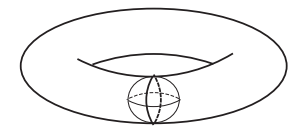
\includegraphics[scale=0.7]{toro1}
\end{figure}
\end{ejercicio}
\begin{solucion}
\end{solucion}

\newpage

\begin{ejercicio}{2.21}
Calcular los $\F$-espacios vectoriales de homología de dos toros entrelazados:

\begin{figure}[h!]
\centering
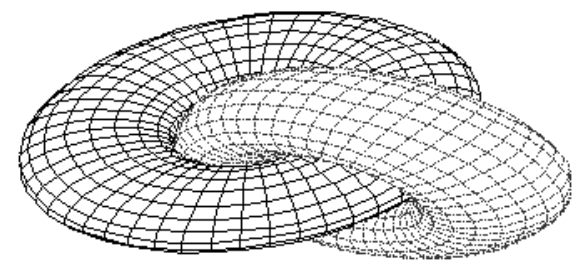
\includegraphics[scale=0.5]{toro2}
\end{figure}
\end{ejercicio}

\begin{solucion}
\end{solucion}

\newpage

\begin{ejercicio}{2.22}
Probar que los espacios euclídeos $\R^n$
y $\R^m$ no son homeomorfos si $n\neq m$.
\end{ejercicio}
\begin{solucion}
Si fueran homeomorfos también serían homeomorfos $\R^n-\{x\}$ y $\R^m-\{y\}$ donde $x\in\R^n$ e $y\in\R^m$. Sabemos que estos espacios son del mismo tipo de homotopía que $S^{n-1}$ y $S^{m-1}$ respectivamente, por lo que conocemos sus espacios de homología, los cuales sabemos que no son iguales si $n\neq m$, por lo que no $\R^n$ no es homeomorfo a $\R^m$ en este caso.
\end{solucion}
\newpage

\begin{ejercicio}{2.23}
Dar un ejemplo de dos espacios topológicos no homeomorfos pero que
tengan todos sus $\F$-espacios vectoriales de homología isomorfos.
\end{ejercicio}
\begin{solucion}
Considerar las realizaciones geométricas de los complejos del ejercicio \ref{ejer:2.4}.
\end{solucion}

\end{document}
